%% 该模板修改自《计算机学报》latex 模板
%% 主要是将双栏改成单栏,去掉了部分计算机学报标识;
%% 源文件自:https://www.overleaf.com/latex/templates/latextemplet-cjc-xelatex/ybmmymncrrmw
%% 
%%
%% This is file `CjC_template_tex.tex',
%% is modified by Zhi Wang (zhiwang@ieee.org) based on the template 
%% provided by Chinese Journal of Computers (http://cjc.ict.ac.cn/).
%%
%% This version is capable with Overleaf (XeLaTeX).
%%
%% Update date: 2023/03/10
%% -------------------------------------------------------------------
%% Copyright (C) 2016--2023 
%% -------------------------------------------------------------------
%% This file may be distributed and/or modified under the
%% conditions of the LaTeX Project Public License, either version 1.3c
%% of this license or (at your option) any later version.
%% The latest version of this license is in
%%    https://www.latex-project.org/lppl.txt
%% and version 1.3c or later is part of all distribution`s of LaTeX
%% version 2008 or later.
%% -------------------------------------------------------------------

\documentclass[10.5pt,compsoc,UTF8]{CjC}
\usepackage{CTEX}
\usepackage{graphicx}
\usepackage{footmisc}
\usepackage{subfigure}
\usepackage{url}
\usepackage{multirow}
\usepackage{multicol}
\usepackage[noadjust]{cite}
\usepackage{amsmath,amsthm}
\usepackage{amssymb,amsfonts}
\usepackage{booktabs}
\usepackage{color}
\usepackage{ccaption}
\usepackage{booktabs}
\usepackage{float}
\usepackage{fancyhdr}
\usepackage{caption}
\usepackage{xcolor,stfloats}
\usepackage{comment}
\setcounter{page}{1}
\graphicspath{{figures/}}
\usepackage{cuted}%flushend,
\usepackage{captionhack}
\usepackage{epstopdf}
\usepackage{gbt7714}
\usepackage{listings}
\usepackage{xeCJK}
\usepackage{float}
\usepackage{sourcecodepro}
\usepackage[T1]{fontenc}
\usepackage{hyperref}

\setmainfont{Times Roman}
% \setCJKmainfont{Noto Sans Mono CJK TC}
\setCJKmainfont{標楷體.ttc}
\setmonofont{Cascadia Code}

%===============================%

\headevenname{\mbox{\quad} \hfill  \mbox{\zihao{-5}{ \hfill 2024 Hardware Design  } \hspace {50mm} \mbox{2024 年 12 月}}}%
\headoddname{Group 21 \hfill Final Project Report}%

%footnote use of *
\renewcommand{\thefootnote}{\fnsymbol{footnote}}
\setcounter{footnote}{0}
\renewcommand\footnotelayout{\zihao{5-}}

\newtheoremstyle{mystyle}{0pt}{0pt}{\normalfont}{1em}{\bf}{}{1em}{}
\theoremstyle{mystyle}
\renewcommand\figurename{figure~}
\renewcommand{\thesubfigure}{(\alph{subfigure})}
\newcommand{\upcite}[1]{\textsuperscript{\cite{#1}}}
\renewcommand{\labelenumi}{(\arabic{enumi})}
\newcommand{\tabincell}[2]{\begin{tabular}{@{}#1@{}}#2\end{tabular}}
\newcommand{\abc}{\color{white}\vrule width 2pt}
\renewcommand{\bibsection}{}
\makeatletter
\renewcommand{\@biblabel}[1]{[#1]\hfill}
\makeatother
\setlength\parindent{2em}
%\renewcommand{\hth}{\begin{CJK*}{UTF8}{gbsn}}
%\renewcommand{\htss}{\begin{CJK*}{UTF8}{gbsn}}
\renewcommand{\contentsname}{Table of Contents}

\begin{document}

\hyphenpenalty=50000
\makeatletter
\newcommand\mysmall{\@setfontsize\mysmall{7}{9.5}}
\newenvironment{tablehere}
  {\def\@captype{table}}

\let\temp\footnote
\renewcommand \footnote[1]{\temp{\zihao{-5}#1}}

\hypersetup{
  colorlinks=false,
  pdfborder={0 0 0},
}

\thispagestyle{plain}%
\thispagestyle{empty}%
\pagestyle{CjCheadings}

% \begin{table*}[!t]
\vspace {-13mm}


\onecolumn
\zihao{5-}\noindent Group 21 \hfill Final Project Report \hfill 2024 年 12 月\\
\noindent\rule[0.25\baselineskip]{\textwidth}{1pt}


\begin{center}
    \vspace {11mm}
    {\zihao{2} \heiti \fangsong Final Project Report}
    
    \vskip 5mm
    
    {\zihao{4}\fangsong Group 21: 陳克盈(112062205)、蔡明妡(112062224)}
\end{center}

\lstset{
    % backgroundcolor=\color{red!50!green!50!blue!50},%程式碼塊背景色為淺灰色
    rulesepcolor= \color{gray}, %程式碼塊邊框顏色
    breaklines=true,  %程式碼過長則換行
    numbers=left, %行號在左側顯示
    numberstyle= \small\ttfamily,%行號字型
    keywordstyle= \color{blue},%關鍵字顏色
    commentstyle=\color{gray}, %註釋顏色
    frame=shadowbox%用方框框住程式碼塊
    basicstyle=\ttfamily\footnotesize,
}
 
\definecolor{improvecolor}{rgb}{0,0.6,0} % 深綠色
\definecolor{declinecolor}{rgb}{0.6,0,0} % 深紅色


%%%%%%%%%%%%%%%%%%%%%%%%%%%%%%%%%%%%%%
\zihao{5}
\vskip 10mm
% \begin{multicols}{1}


%%%%%%%%%%%%%%%%%%%%%%%%%%%%%%%%%%%%%%%%%%
%%%%%%%%%%%%%%%%%%%%%%%%%%%%%%%%%%%%%%%%%%

\tableofcontents
\newpage

\section{Introduction}

\subsection{Motivation}
近期比特幣已經突破九萬美元,市值已經突破 9000 年以來所開採的白銀總值,成為全球第八大資產。\
雖然距離全就第一大資產黃金還有很大一段距離,但是從近期走勢,以及加密貨幣 ETF 的興起,\
都顯示加密貨幣已經成為投資者的一大選擇。

近年來高頻交易在金融市場的佔比日益增長,根據研究報導 \footnote{https://www.investopedia.com/terms/h/high-frequency-trading.asp}指出,\
高頻交易在美國股市的交易量佔比穩定在 50\% 以上,而歐洲股市 \footnote{https://www.ecb.europa.eu/press/research-publications/resbull/2020/html/ecb.rb201215~210477c6b0.en.html} \
的佔比則在 24 - 43\% 左右。\

有別於傳統股票市場有著交易所開盤時間的限制,加密貨幣是全球化且全年無休的市場,\
這也使得加密貨幣成為高頻交易的首選,目前高頻交易佔加密貨幣交易所的交易量穩定在 50\% \footnote{https://blog.ueex.com/cryptocurrency-high-frequency-trading-tactics/} 以上,\
其中中國市場更是高達 60 - 80 \% 以上 \footnote{https://www.investopedia.com/news/highfrequency-trading-firms-enter-cryptocurrency-markets/}。

高頻交易除了一般的程式交易之外,也有不少造市商使用 FPGA 能夠實現硬體加速的特性來近一步地降低計算延遲。\
雖然我們無法取得 PCIE 等級的 FPGA 板,但我們仍然能夠使用 FPGA 來模擬高頻交易的環境,這也是為什麼我們選擇這個題目作為我們的 Final Project。

\subsection{Overall Introduction}
在這個專案中,交易將會有兩種模式:
\begin{itemize}
  \item 手動模式:透過鍵盤輸入,模擬交易員手動下單的情況。
  \item 自動模式:FPGA 將會內建幾個自動交易策略,FPGA 讀取交易資料後,\
  便會根據策略發出買賣指令。
\end{itemize}

這兩種模式都將使用 FPGA 作為 IO 與計算的核心,並使用電腦與 FPGA 連接,作為網路封包的傳輸跳板,\
將對應的 API Request 傳送到 Binance 交易所進行交易,以下是使用者能夠進行的操作:

\begin{itemize}
  \item 鍵盤輸入:
  \begin{itemize}
    \item 輸入 BUY(或是 B)、SELL(或是 S)、CLOSE(或是 C),並在後面加上 BTC / ETH 來進行買入、賣出、平倉,以空格隔開。\
    在後面加上 at 價格時能夠進行限價交易
    \item 輸入 QUERY 來查詢目前帳戶的資訊
    \item 輸入 LEVERAGE 來更改槓桿倍數
  \end{itemize}
\end{itemize}
\newpage
\begin{itemize}
  \item FPGA 操作:
  \begin{itemize}
    \item 按鈕:上鍵代表買入、中鍵代表平倉、下鍵代表賣出
    \item 最右邊的開關:交易 BTC / ETH
    \item 右二開關:是否開啟自動交易,若開啟自動交易,FPGA 會根據策略,每兩秒鐘根據目前資料進行交易訊號的判定,並在損益超過正負 20\% 時進行平倉
  \end{itemize}
\end{itemize}

\section{架構}

\subsection{整體架構}

在手動模式下,機器的運作模式主要分成了幾個步驟:
\begin{enumerate}
  \item FPGA 讀取鍵盤輸入,並將輸入內容透過 MicroUSB 傳送到 Host 端
  \item 當 Enter 鍵被按下時,Host 端的 Buffer 會將指令傳送到 API Request Generator 並轉換成對應的 API Request
  \item API Request 透過 Binance API 送到 Binance 交易所,完成一次交易
\end{enumerate}

在自動模式下,策略模組將會介入交易行為:

\begin{enumerate}
  \item 策略模組定時透過 MicroUSB 向 Host 端發送查詢目前價格、成交量、倉位損益等資訊
  \item Host 端接收到 FPGA 的查詢後,將會透過 Binance API 取得對應的資訊
  \item Host 端將資訊傳送到 FPGA,FPGA 根據策略模組的設定,決定是否要進行交易
  \item 策略模組透過 MicroUSB 向 Host 端發送交易指令,完成一次自動交易
\end{enumerate}

\begin{figure}[H]
  \centering
  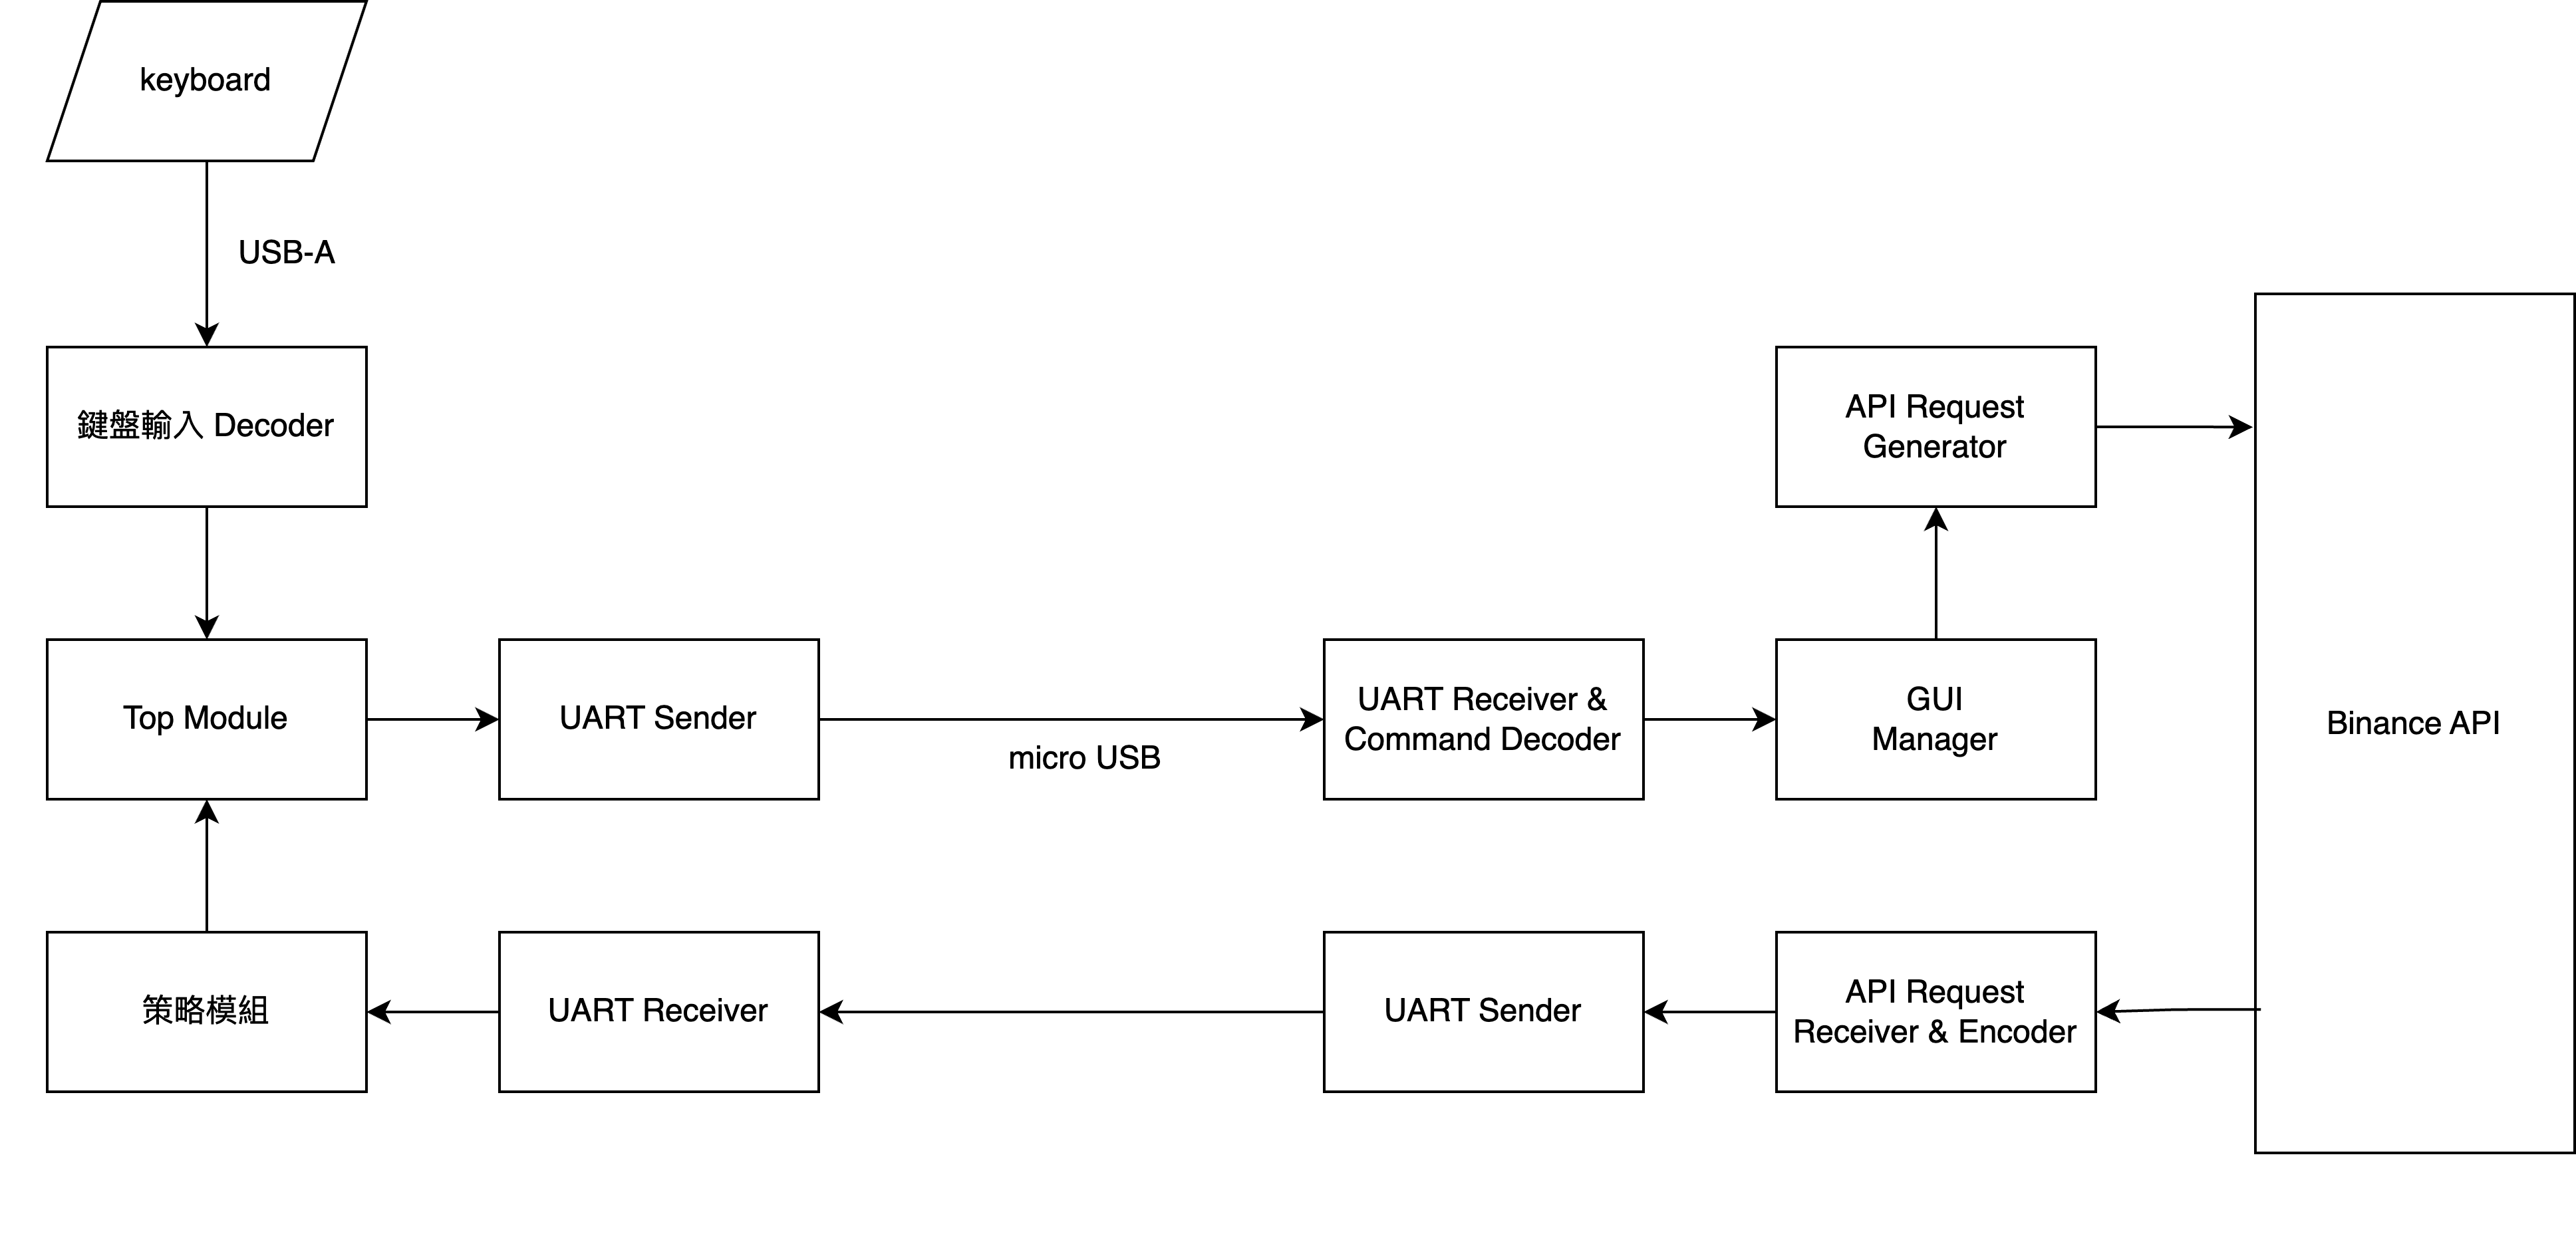
\includegraphics[width=\textwidth]{./img/arch.png}
  \caption{整體架構}
\end{figure}

\subsection{FPGA 模組細節}

\subsubsection*{Top Module}

Top Module 負責串接並控制所有模組,並且內建一個 Queue,用來儲存準備要透過 UART 傳送的資料,主要功能如下。

\begin{itemize}
  \item 接收來自 Keyboard Decoder 的輸入
  \item 接收來自 FPGA 按鍵的輸入
  \item 將需要被發送的資料儲存到 Queue 中,並在空閒時透過 UART 傳送到 Host 端
  \item 接收來自自動交易模組的訊號,並將對應的 Binary Code 發送出去
\end{itemize}

\subsubsection*{Keyboard Decoder}

\begin{itemize}
  \item 讀取鍵盤輸入
  \item 支援 Enter, Backspace, Delete, 上下左右等按鍵
  \item 將輸入內容傳送至 Top Module
\end{itemize}

\subsubsection*{UART Module}
UART (Universal Asynchronous Receiver/Transmitter) 每次能夠傳送 8 bits 的資料,\
在傳送之前,訊號會一直保持在高電位,當要傳送資料時,會將訊號變為低電位一個 clock cycle,\
代表開始傳輸,接著依序傳送 8 bits 的資料,最後再將訊號拉回高電位代表 stop bit 來表示傳輸結束,如下圖所示。

\begin{figure}[H]
  \centering
  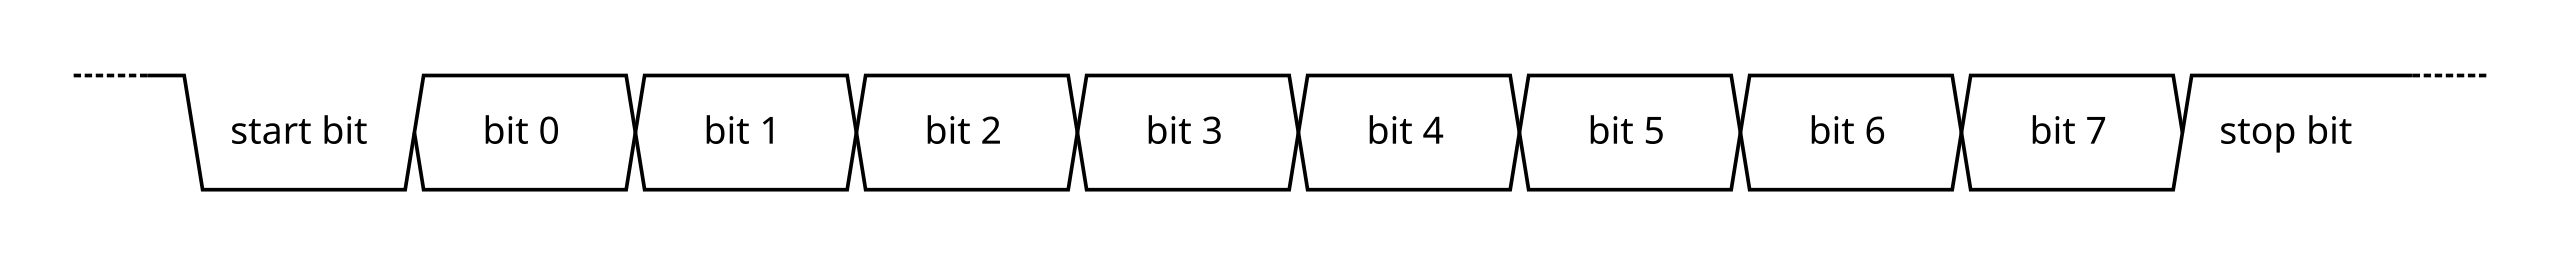
\includegraphics[width=\textwidth]{./img/UART.png}
  \caption{UART 傳輸流程}
\end{figure}

\begin{figure}[H]
  \centering
  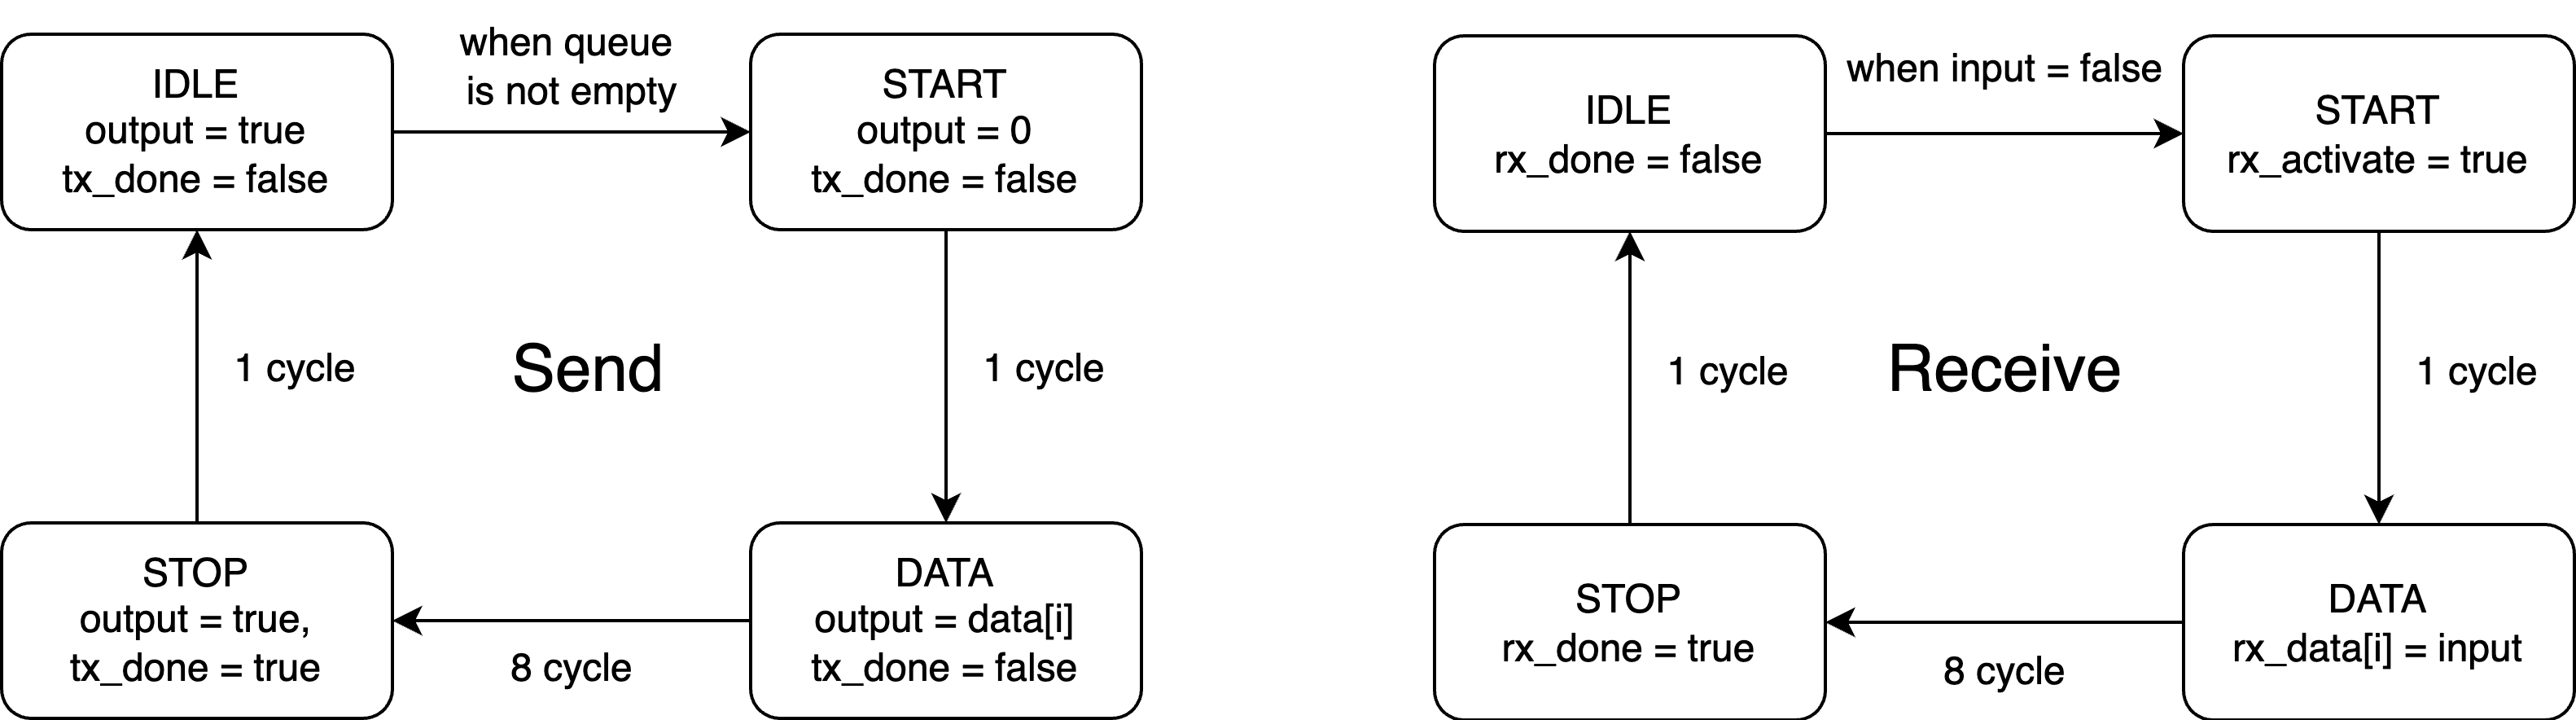
\includegraphics[width=\textwidth]{./img/UART-State.png}
  \caption{UART State Diagram}
\end{figure}

為了避免有多組訊號同時需要被送出,在 UART 模組中內建了一個 Queue,用來儲存準備要被送出的資料。

\subsubsection*{Queue}

與課堂中寫到的 Queue 相似,接收以下幾種參數:
\begin{itemize}
  \item wen: 是否有新的資料要被寫入
  \item ren: 是否要從 Queue 中 pop 資料
  \item argc: 要被寫入的資料有幾個
  \item din1, din2, din3, din4: 要被寫入的資料
  \item dout: 被 pop 出來的資料
  \item empty, full: Queue 是否為空或滿
\end{itemize}

Top 模組會根據以下的行為,對 Queue 與 UART 端進行操作:

\begin{itemize}
  \item 鍵盤輸入:向 UART Module 發送 0x01 的 prefix byte,並將鍵盤輸入的 ASCII Code 放入 Queue 中
  \item 買、賣、平倉:向 UART Module 發送 0x02(買)、0x03(賣)、0x04(平倉)的 prefix byte,\
        並將交易對編號 0x01 (BTC), 0x02 (ETH) 放入 Queue 中
  \item 當 clock counter 數到奇數秒,向 UART Module 發送 0x05 的 prefix byte,\
        並將將交易對編號 0x01 (BTC), 0x02 (ETH) 放入 Queue 中,代表查詢近五分鐘的 K 棒資料
  \item 當 clock counter 數到偶數秒,向 UART Module 發送 0x06 的 prefix byte,\
        並將將交易對編號 0x01 (BTC), 0x02 (ETH) 放入 Queue 中,代表查詢該交易對目前倉位的損益
\end{itemize}

\subsubsection*{策略模組}
策略模組主要會接收 UART Receiver 得到的資料,並進行停損停利以及買賣訊號的判斷。我們將這個過程分成了五個 State:

\begin{itemize}
  \item State 0:等待接收資料,當 input\_done 訊號為 1 時,會判斷目前接收到的資料(prefix byte)是什麼,\
        prefix\_byte 為 0x01 時代表接收到了 K 線的資料,進入到 State 1。0x02 則是接收到目前倉位的損益,進入到 State 3。
  \item State 1:接收 K 線資料,這個階段會接收五組的 K 線資料,每組資料包含以下資訊。在接收 80 byte 的資料後,進入 State 2。
  \begin{itemize}
    \item timestamp: 8 bits,代表這組 K 線的時間戳
    \item open\_price: 24 bits,代表這組 K 線的開盤價
    \item high\_price: 24 bits,代表這組 K 線的最高價
    \item low\_price: 24 bits,代表這組 K 線的最低價
    \item close\_price: 24 bits,代表這組 K 線的收盤價
    \item volume: 24 bits,代表這組 K 線的成交量
  \end{itemize}
  \item State 2:計算交易訊號,這個階段會計算出當前的 MA5(近 5 分鐘的平均價格)、momentum(價格動量方向),並根據以上資料計算出買賣訊號:
  \begin{itemize}
    \item 買入:目前價格大於 MA5、動量朝上、成交量增加百分之十、突破前 K 棒高點,這四個條件滿足其中三個以上時買入
    \item 賣出:目前價格小於 MA5、動量朝下、成交量減少百分之十、突破前 K 棒低點,這四個條件滿足其中三個以上時賣出
  \end{itemize}
  \item State 3:接收帳戶資料,這個階段會接收一個 8 bit 的有號整數,代表目前倉位的損益率,並進入 State 4。
  \item State 4:計算停損停利,這個階段會根據目前倉位的損益率,當損益率的絕對值超過 20\% 時,會發出平倉訊號。
\end{itemize}

\begin{figure}[!h]
  \centering
  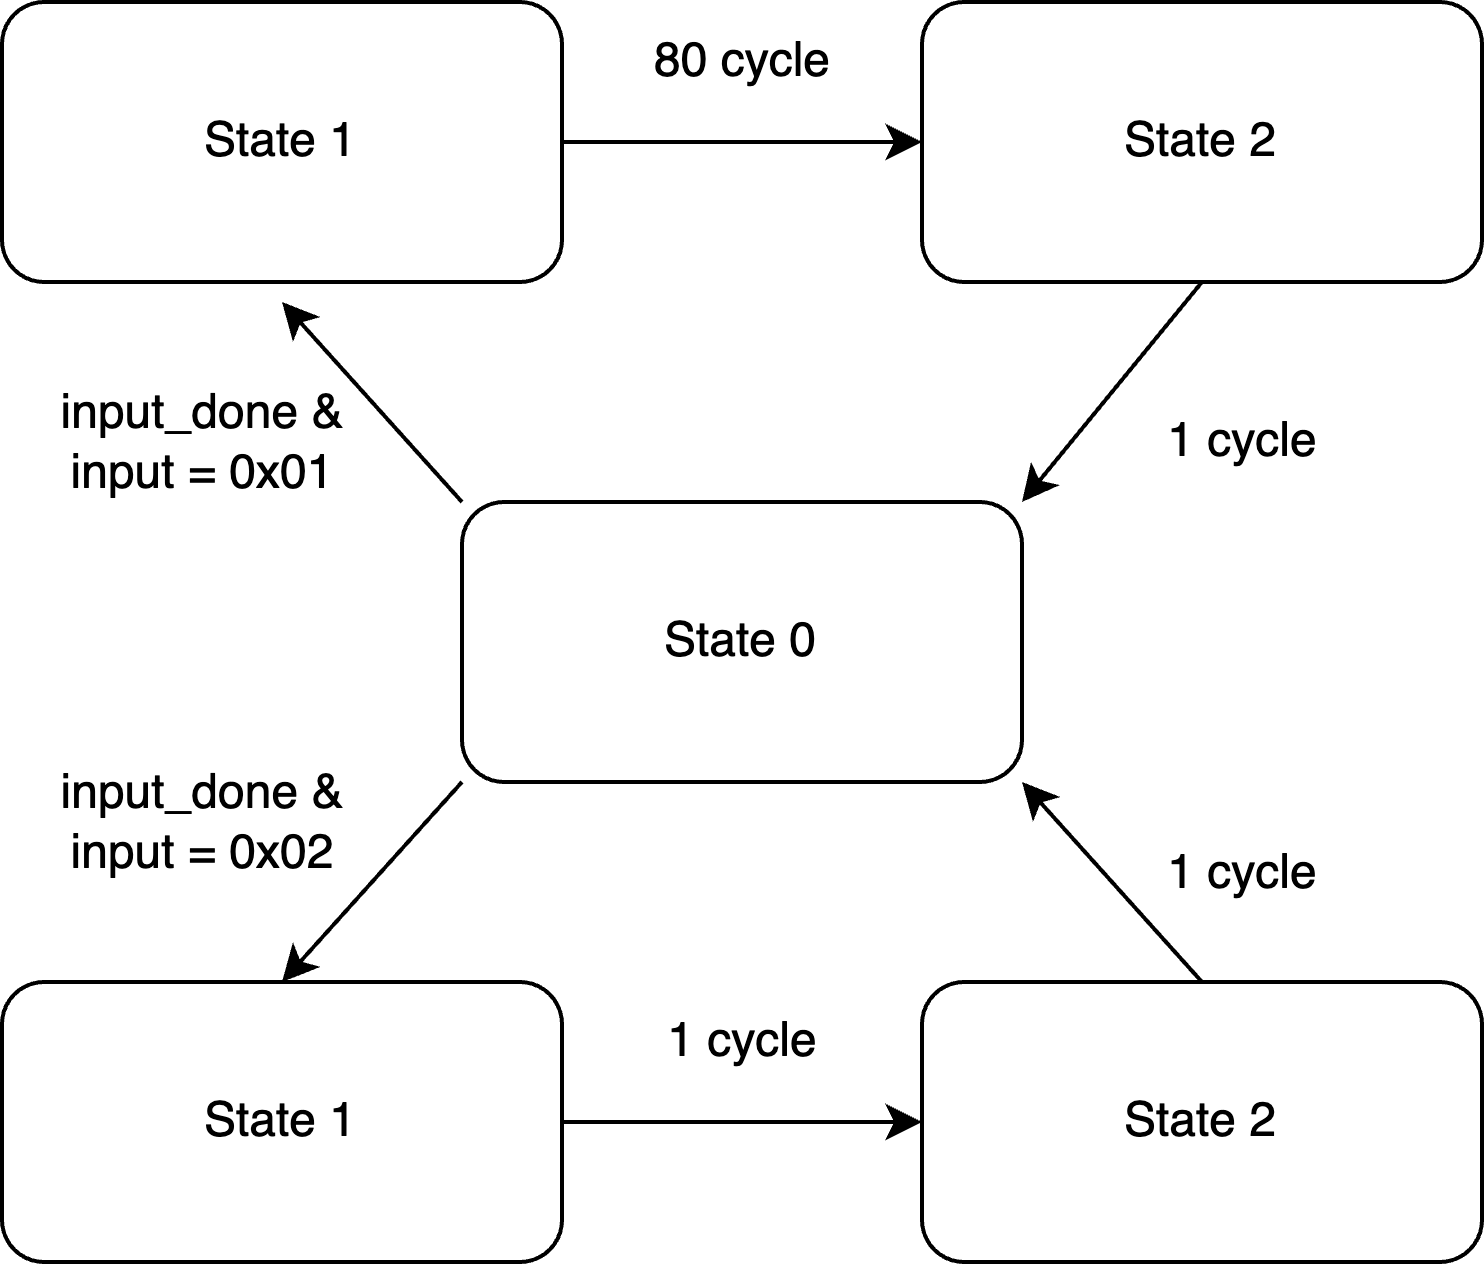
\includegraphics[width=0.7\textwidth]{./img/Trade.png}
  \caption{Trading State Diagram}
\end{figure}

\subsection{Host 端模組細節}

\subsubsection*{UART Receiver \& Command Decoder}
這部分會接收由 FPGA 發送的資料,根據 prefix byte 來判斷接收到的指令類型是什麼後,\
根據接收到的第二個 byte 來判斷指令內容,並將這兩個資訊打包後,透過 websocket 傳送給 GUI。

\subsubsection*{GUI}
GUI 會啟動一個終端機模擬器,模擬平常使用終端機打指令的場景,並將鍵盤輸入的內容顯示在終端機上,並將指令轉發給 API Request Generator,根據不同資料會分成兩種操作:
\begin{itemize}
  \item 鍵盤輸入:由於 ASCII 本身不支援上下左右之類的按鍵,因此我額外指定了一些 Code 代表特殊操作:
  \begin{itemize}
    \item 0x01: UP:切換到上一條指令
    \item 0x02: DOWN:切換到下一條指令
    \item 0x03: LEFT:游標左移
    \item 0x04: RIGHT:游標右移
    \item 0x08: Backspace
    \item 0x7F: Delete
    \item 0x0D: Enter,按下 Enter 後,會再進行一次 Command Decode,將輸入的資料轉為指定的指令格式,再傳送到 API Request Generator
  \end{itemize}
  \item 買、賣、平倉:將 log 顯示在終端機模擬器中,並將指令透過 websocket 傳送到 API Request Generator 中
\end{itemize}

\subsubsection*{API Request Generator、API Request Receiver}
這裡將會接收 GUI 傳來的指令資訊,並將其轉換成對應的 API Request,包含以下幾種指令:
\begin{itemize}
  \item 市價買入、市價賣出
  \item 限價買入、限價賣出
  \item 平倉
  \item 查詢近五分鐘的 K 棒資料
  \item 查詢目前倉位的損益
  \item 查詢目前倉位的資訊
  \item 更改槓桿倍數
\end{itemize}

以上的指令中,查詢近五分鐘的 K 棒資料以及查詢目前倉位的損益,是需要回傳給 FPGA 的,\
此時便會呼叫 UART 的 Sender,將 API 回傳的資料傳送給 FPGA:
\begin{itemize}
  \item 查詢近五分鐘的 K 棒資料:將近五分鐘的 K 棒資料,每 8 個 byte 為一組,搭配 prefix byte 0x01 傳送給 FPGA
  \item 將目前倉位的損益,以 8 bit 的有號整數格式,搭配 prefix byte 0x02 傳送給 FPGA
\end{itemize}

\subsection{實驗結果}

在手動模式之下,透過 FPGA 上的按鈕來進行交易,能夠有效地將交易的時間,從原先使用 APP 的 1 ~ 2 秒縮短到不到半秒鐘即可成功下單。\
\par
而在自動模式之下,在完全不介入交易、完全透過 FPGA 判斷買賣的情況下,成功的完成數筆交易,並且具有一定的交易勝率

\begin{figure}[h!]
  \centering
  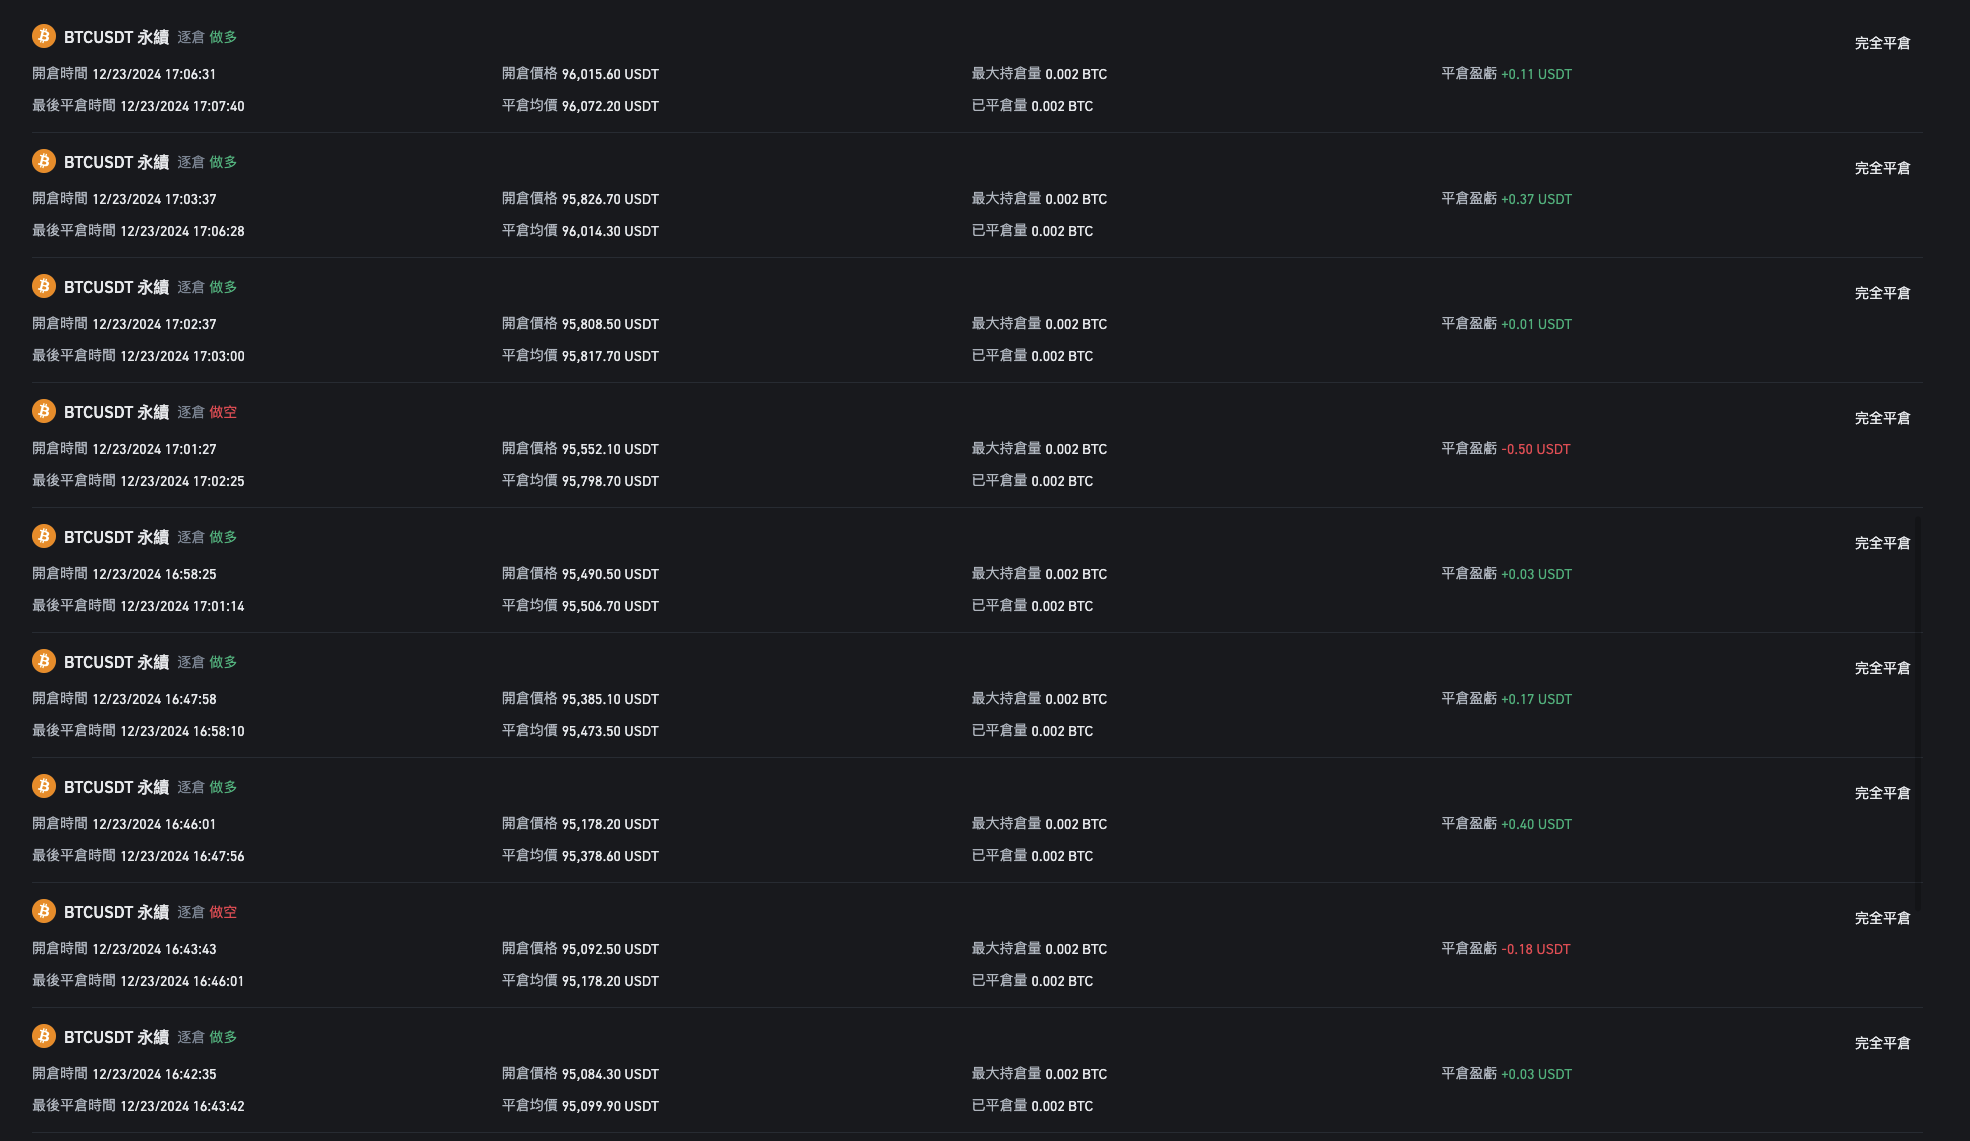
\includegraphics[width=\textwidth]{./img/trade-history.png}
  \caption{交易結果}
\end{figure}

\end{document}


